%=================================================================
% MIT LICENSE
%=================================================================
% Copyright (c) 2022 Techneatium
%
% Permission is hereby granted, free of charge, to any person obtaining a copy
% of this software and associated documentation files (the "Software"), to deal
% in the Software without restriction, including without limitation the rights
% to use, copy, modify, merge, publish, distribute, sublicense, and/or sell
% copies of the Software, and to permit persons to whom the Software is
% furnished to do so, subject to the following conditions:
%
% The above copyright notice and this permission notice shall be included in all
% copies or substantial portions of the Software.
%
% THE SOFTWARE IS PROVIDED "AS IS", WITHOUT WARRANTY OF ANY KIND, EXPRESS OR
% IMPLIED, INCLUDING BUT NOT LIMITED TO THE WARRANTIES OF MERCHANTABILITY,
% FITNESS FOR A PARTICULAR PURPOSE AND NONINFRINGEMENT. IN NO EVENT SHALL THE
% AUTHORS OR COPYRIGHT HOLDERS BE LIABLE FOR ANY CLAIM, DAMAGES OR OTHER
% LIABILITY, WHETHER IN AN ACTION OF CONTRACT, TORT OR OTHERWISE, ARISING FROM,
% OUT OF OR IN CONNECTION WITH THE SOFTWARE OR THE USE OR OTHER DEALINGS IN THE
% SOFTWARE.
%=================================================================

%-----------------------------------------------------------------
% BEGIN DOCUMENT
%-----------------------------------------------------------------
\documentclass[fontInter]{TechCheck}
\title{AH64_Cheatsheet}
\author{Techneatium}

\setaircraftlong{AH-64D AIRCRAFT} % sets long label for title page
\setaircraftshort{AH-64D} % sets short label for header
\settabnumber{8} % sets number of tabs for document

\begin{document}
	%-----------------------------------------------------------------
% TITLE PAGE
%-----------------------------------------------------------------
	% deactivate header and footer
	\pagestyle{empty}
	\newlength{\centeroffset}
	\setlength\centeroffset{(\chevin-\outmar-0.5cm)/2}
	\begin{tikzpicture}[overlay, remember picture]
	\node[
	]() at ([xshift=\centeroffset,yshift=8.5cm]current page.center) {
		\Huge \titlefont\textbf{Pocket Checklist}
	};
	\node[
	]() at ([xshift=\centeroffset,yshift=7cm]current page.center) {
		\resizebox{10cm}{!}{\titlefont\textbf{\colorbox{color1}{\textcolor{white}{\aircraftlong}}}}
	};
	\node[
	]() at ([xshift=\centeroffset,yshift=5.5cm]current page.center) {
		\Large \titlefont\textbf{\colorbox{color1}{\textcolor{white}{REV: \today}}} \blue{}
	};
	\node[
	]() at ([xshift=\centeroffset,yshift=-1cm]current page.center) {
		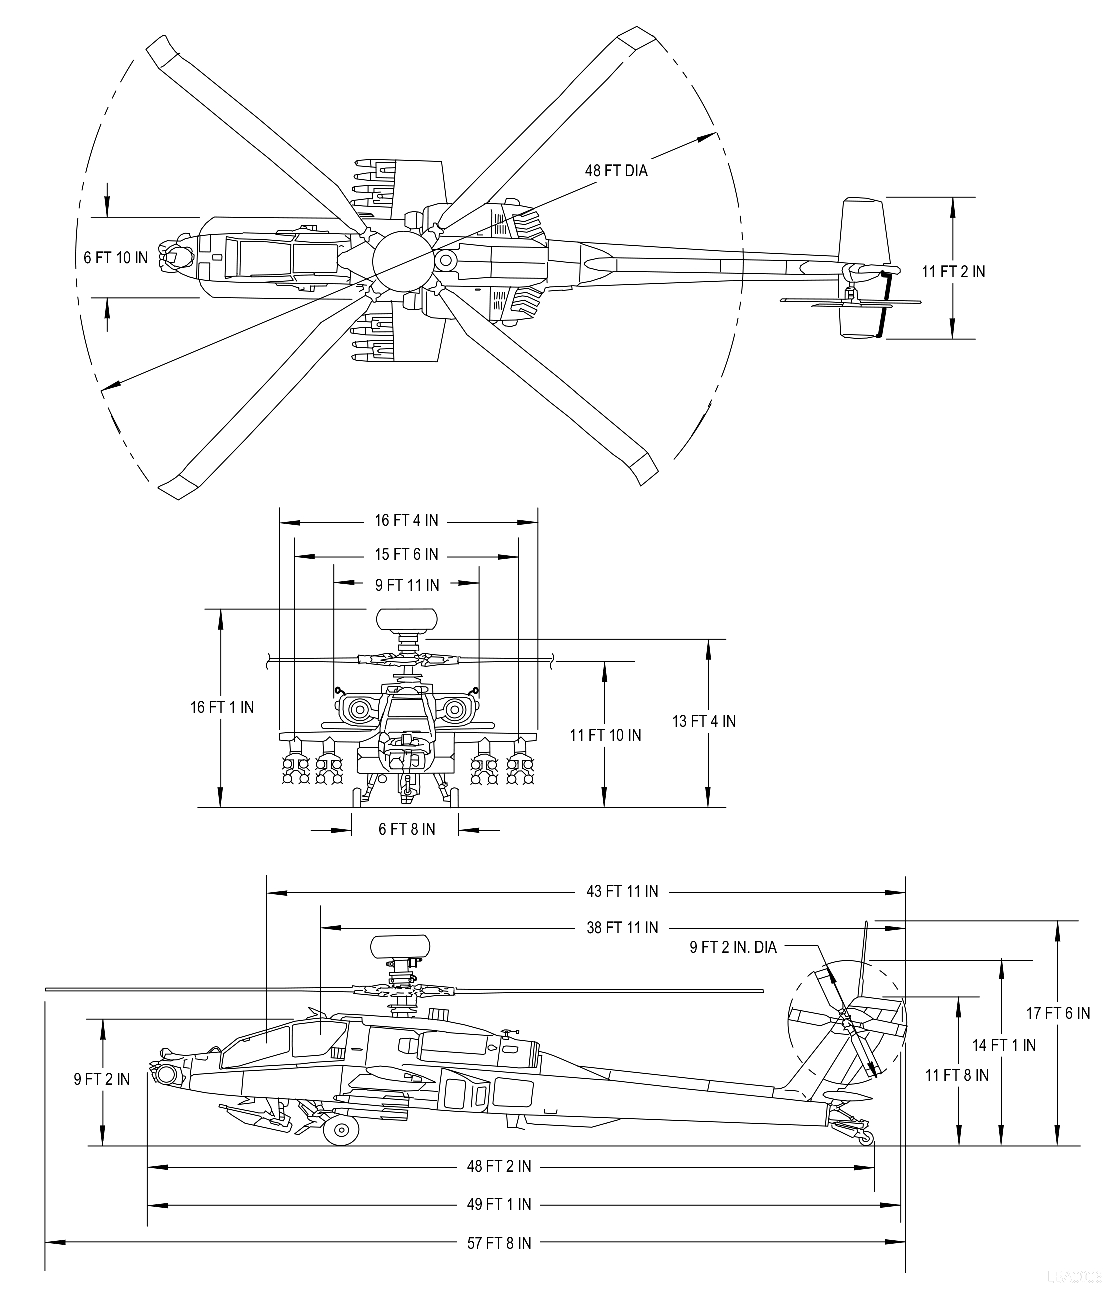
\includegraphics[
			width=0.75\linewidth,
			% page = {1},
			% trim = {3cm, 10.5cm, 6.5cm, 13.5cm},
			% clip
		]{Apache_dimensions.pdf}
	};
	% Black area for white chevrons
	\fill[color1]
		([xshift=\outmar, yshift=0.2cm]current page text area.north east) --
		([xshift=\outmar, yshift=-\botmar]current page text area.south east) --
		([xshift=\chevin-0.5cm, yshift=-\botmar]current page text area.south east) --
		([xshift=\chevin-0.5cm, yshift=0.2cm]current page text area.north east) --
		cycle;
	\end{tikzpicture}
	% label for hyperrefs back to frontpage
	\label{frontpage}
	% make chevrons
	\thumbfront{Procedures}{0}
	% \thumbfront{Systems}{1}
	% % use tabular for multi line node
	% \thumbfront{\begin{tabular}{c} APG-68 \\ FCR \end{tabular}}{2}
	% \thumbfront{\begin{tabular}{c} LITENING \\ TGP \end{tabular}}{3}
	% \thumbfront{\begin{tabular}{c} A/G \\ Weapons \end{tabular}}{4}
	% \thumbfront{\begin{tabular}{c} A/A \\ Weapons \end{tabular}}{5}
	\thumbwide

	\clearpage
	\null\vspace{0cm}

	\begin{tcolorbox}[
		enhanced, colback=white, colframe=color1, colbacktitle=white, coltitle=color1, sharp corners, attach boxed title to top center={yshift=2mm},
		boxed title style={
			sharp corners,
			drop shadow=color1!100
		}, title=\LARGE\textbf{DISCLAIMER}
	]
		\textbf{This document represents a personal project and is intended for entertainment purposes only. Do not use for training purposes or in real life scenarios.}
	\end{tcolorbox}

	\cleardoublepage

	\thumbnar
	\dominitoc
	\tableofcontents
	\cleardoublepage

	% restart page counter
	\setcounter{page}{1}
	% reactivate header and footer
	\pagestyle{body}

	\chapter{PROCEDURES}
	\thumbtab{Procedures}{0}
	\minitoc
	\cleardoublepage

	\section{START-UP}

	\subsection{INTERIOR CHECKS}
	\begin{tableitemize}
		\blueitem{Canopy Door (PLT/CPG)}{\textbf{As Desired}}
		\midrule
		\multicolumn{3}{c}{\textbf{LEFT SIDE -- BACK TO FRONT}} \\
		\blueitem{Lights Panel (PLT/CPG)}{
		\begin{subitemize}
			\item \textbf{EXT LT/INTR LT Panel} \dotfill \textbf{As Required} \\
			\emph{(PLT)}
			\item \textbf{INTR LT Panel} \dotfill \textbf{As Required} \\
			\emph{(CPG)}
		\end{subitemize}}
		\blueitem{Power Levers (PLT/CPG)}{\textbf{OFF}}
		\blueitem{ENG START Switches (PLT)}{\textbf{OFF}}
		\blueitem{RTR BRK Switch (PLT)}{\textbf{OFF}}
		\blueitem{NVS MODE Switch (PLT/CPG)}{\textbf{OFF}}
		\midrule
		\multicolumn{3}{c}{\textbf{FRONT PANEL -- LEFT TO RIGHT}} \\
		\blueitem{KU Brightness Knob (PLT/CPG)}{\textbf{As Desired}}
		\blueitem{VIDEO Panel (PLT)}{\textbf{Knobs at 12 o'clock}}
		\blueitem{MPD/EUFD Brightness Knob (PLT/CPG)}{\textbf{As Desired}}
		\blueitem{CMWS (PLT)}{
		\begin{subitemize}
			\item \textbf{CMWS Control Indicator PWR} \dotfill \textbf{OFF}
			\item \textbf{CMWS/NAV Switch} \dotfill \textbf{CMWS}
			\item \textbf{BYPASS/AUTO Switch} \dotfill \textbf{AUTO}
			\item \textbf{JETTISON Switch} \dotfill \textbf{OFF}
		\end{subitemize}}
		\blueitem{TEDAC R Grip LT (CPG)}{\textbf{OFF}}
		\blueitem{PARK BRAKE (PLT)}{\textbf{SET}, Handle out}
		\blueitem{Standby Instruments (PLT)}{\textbf{Check}, caged}
		\midrule
		\multicolumn{3}{c}{\textbf{RIGHT SIDE -- FRONT TO BACK}} \\
		\blueitem{COMM Panel (PLT/CPG)}{\textbf{As Desired}}
		\blueitem{HDU (PLT/CPG)}{\textbf{As Desired}}
	\end{tableitemize}

	\clearpage

	\subsection{APU-START}
	\begin{tablenumerate}
		\multicolumn{3}{c}{\textbf{PRE APU START}} \\
		\midrule
		\blueitem{MSTR IGN Switch (PLT)}{\textbf{BATT}}
		\blueitem{Searchlight (PLT)}{\textbf{As Required}}
		\blueitem{TAIL WHEEL Button (PLT)}{\textbf{Locked}, UNLOCKED Light is off}
		\blueitem{EMERG HYD Button (PLT/CPG)}{Verify \textbf{ON Light} not illuminated}
		\blueitem{Cautions (PLT/CPG)}{\textbf{Check MSTR WARN, MSTR CAUT, EUFD}}
		\blueitem{Fire Test (PLT/CPG)}{
		\begin{subenumerate}
			\item \textbf{FIRE DET/EXTG TEST} \dotfill \textbf{Position 1} (PLT)
			\item \textbf{FIRE DET/EXTG TEST} \dotfill \textbf{Position 2} (CPG)
		\end{subenumerate}

		\emph{In each position, both crewmembers should check the following}
		\begin{subitemize}
			\item \textbf{MSTR WARN} \dotfill \textbf{illuminated}
			\item \textbf{ENG 1 FIRE} \dotfill \textbf{illuminated}
			\item \textbf{APU FIRE} \dotfill \textbf{illuminated}
			\item \textbf{ENG 2 FIRE} \dotfill \textbf{illuminated}
			\item \textbf{AFT DECK FIRE} \dotfill EUFD Warning
			\item \textbf{Voice Warning System} \dotfill activates
		\end{subitemize}}
		\midrule
		\multicolumn{3}{c}{\blue{APU START}} \\
		\blueitem{APU (PLT)}{
		\begin{subenumerate}
			\item \textbf{APU Button} \dotfill \textbf{Press \& Release}
			\item \textbf{EUFD} \dotfill \textbf{Observe Advisories}
			\begin{itemize}
				\item \textbf{APU START}
				\item \textbf{APU POWER ON}
				\item \textbf{ACCUM OIL PRESS LO}
			\end{itemize}
		\end{subenumerate}}
		\midrule
		\multicolumn{3}{c}{\textbf{POST APU START}} \\
		\blueitem{Canopy (PLT/CPG)}{\textbf{As Desired}}
		\blueitem{DTU Page (PLT/CPG)}{\textbf{Select Load}}
		\blueitem{Menu Page (PLT/CPG)}{\textbf{Perform DMS Sweep}}
	\end{tablenumerate}

	\notebox{
		\begin{itemize}
			\item \textbf{Recommended DMS Sweep Technique: Clockwise from top right of any page}
			\begin{itemize}
				\item Exact sweep may vary based on mission requirements
			\end{itemize}
			\item \textbf{Recommended MPD Setup:} \textbf{Right MPD} set to TSD, \textbf{Left MPD} used as \emph{``Working MPD''}
		\end{itemize}
	}

	\subsection{ENGINE-START}
	\begin{tablenumerate}
		\multicolumn{3}{c}{\blue{PRE ENGINE START}} \\
		\blueitem{NVS Mode Switch (PLT/CPG)}{\textbf{As Desired}}
		\blueitem{Standby ADI (PLT)}{\textbf{Uncage}}
		\midrule
		\multicolumn{3}{c}{\blue{ENGINE START}} \\
		\blueitem{RTR BRK Switch (PLT)}{\textbf{OFF}  or \textbf{LOCK} for rotor lock start}
		\blueitem{EXT LT ANTI COL (PLT)}{\textbf{WHT} for day, \textbf{RED} for night}
		\blueitem{ENG 1 Start (PLT)}{
		\begin{subenumerate}
			\item \textbf{ENG 1 START Switch} \dotfill \textbf{START}
			\item \textbf{EUFD} \dotfill \textbf{ENG 1 START}
			\item \textbf{ENG TGT} \dotfill < 80 deg C
			\item \textbf{Power Lever} \dotfill \textbf{IDLE}
			\item \textbf{Monitor}
			\begin{itemize}
				\item \textbf{TGT}
				\item \textbf{NG}
				\item \textbf{MSTR WARN/CAUT}
				\item \textbf{EUFD}
			\end{itemize}
		\end{subenumerate}}
		\blueitem{ENG 2 Start (PLT)}{
		\begin{subenumerate}
			\item \textbf{ENG 2 START Switch} \dotfill \textbf{START}
			\item \textbf{EUFD} \dotfill \textbf{ENG 2 START}
			\item \textbf{ENG TGT} \dotfill < 80 deg C
			\item \textbf{Power Lever} \dotfill \textbf{IDLE}
			\item \textbf{Monitor}
			\begin{itemize}
				\item \textbf{TGT}
				\item \textbf{NG}
				\item \textbf{MSTR WARN/CAUT}
				\item \textbf{EUFD}
			\end{itemize}
		\end{subenumerate}}
		\blueitem{RTR BRK Switch (PLT)}{\textbf{OFF}}
		\blueitem{Stabilized Parameters (PLT)}{
		\begin{subitemize}
			\item \textbf{ENG 1 \& 2 OIL PRES} -- < 70 PSI
			\item \textbf{NGB TEMP} -- > 20 deg C
		\end{subitemize}}
		\blueitem{Power Levers (PLT)}{Advance smoothly to \textbf{FLY}}
		\blueitem{NP \& NR (PLT)}{Verify 101\%}
		\blueitem{APU (PLT)}{\textbf{OFF}}
	\end{tablenumerate}

	\subsection{PRE-TAXI}
	\begin{tablenumerate}
		\blueitem{EXT LT Panel (PLT)}{Verify \textbf{NAV} lights set to \textbf{BRT}, \textbf{ANTI-COL} Set as required}
		\blueitem{Searchlight (PLT/CPG)}{\textbf{As Required}}
		\blueitem{PARKING BRAKE (PLT)}{\textbf{Released}, Handle in}
		\blueitem{TAIL WHEEL Button (PLT)}{\textbf{UNLOCK} as desired}
	\end{tablenumerate}

	\cleardoublepage

	\section{START-UP (ITEMIZE)}

	\subsection{INTERIOR CHECKS}
	\begin{itemize}[leftmargin=0.1\linewidth,rightmargin=0.1\linewidth, itemsep=4pt]
		\item \blue{Canopy Door} \textbf{(PLT/CPG)} \dotfill \textbf{As Desired}
		\item \blue{Lights Panel} \textbf{(PLT/CPG)} 
		\begin{itemize}[itemsep=4pt]
			\item \textbf{EXT LT/INTR LT Panel} \dotfill \textbf{As Required}
			\emph{(PLT)}
			\item \textbf{INTR LT Panel} \dotfill \textbf{As Required}
			\emph{(CPG)}
		\end{itemize}
		\item \blue{Power Levers} \textbf{(PLT/CPG)} \dotfill \textbf{OFF}
		\item \blue{ENG START Switches} \textbf{(PLT)} \dotfill \textbf{OFF}
		\item \blue{RTR BRK Switch} \textbf{(PLT)} \dotfill \textbf{OFF}
		\item \blue{NVS MODE Switch} \textbf{(PLT/CPG)} \dotfill \textbf{OFF}
		\item \blue{KU Brightness Knob} \textbf{(PLT/CPG)} \dotfill \textbf{As Desired}
		\item \blue{VIDEO Panel} \textbf{(PLT)} \dotfill \textbf{Knobs at 12 o'clock}
		\item \blue{MPD/EUFD Brightness Knob} \textbf{(PLT/CPG)} \dotfill \textbf{As Desired}
		\item \blue{CMWS} \textbf{(PLT)}
		\begin{itemize}[itemsep=4pt]
				\item \textbf{CMWS Control Indicator PWR} \dotfill \textbf{OFF}
				\item \textbf{CMWS/NAV Switch} \dotfill \textbf{CMWS}
				\item \textbf{BYPASS/AUTO Switch} \dotfill \textbf{AUTO}
				\item \textbf{JETTISON Switch} \dotfill \textbf{OFF}
		\end{itemize}
		\item \blue{TEDAC R Grip LT} \textbf{(CPG)} \dotfill \textbf{OFF}
		\item \blue{PARK BRAKE} \textbf{(PLT)} \dotfill \textbf{SET}, Handle out
		\item \blue{Standby Instruments} \textbf{(PLT)} \dotfill \textbf{Check}, caged
		\item \blue{COMM Panel} \textbf{(PLT/CPG)} \dotfill \textbf{As Desired}
		\item \blue{HDU} \textbf{(PLT/CPG)} \dotfill \textbf{As Desired} \\
	\end{itemize}

	\clearpage

	\subsection{APU-START}
	\begin{enumerate}[leftmargin=0.1\linewidth,rightmargin=0.1\linewidth, itemsep=4pt]
		\item \blue{MSTR IGN Switch} \textbf{(PLT)}\cbstart \dotfill \textbf{BATT}\cbend
		\item \blue{Searchlight} \textbf{(PLT)} \dotfill \textbf{As Required}
		\item \blue{TAIL WHEEL Button} \textbf{(PLT)} \dotfill \textbf{Locked}, UNLOCKED Light is off
		\item \blue{EMERG HYD Button} \textbf{(PLT/CPG)} \dotfill Verify \textbf{ON Light} not illuminated
		\item \blue{Cautions} \textbf{(PLT/CPG)} \dotfill \textbf{Check MSTR WARN, MSTR CAUT, EUFD}
		\item \blue{Fire Test} \textbf{(PLT/CPG)} 
		\begin{enumerate}[itemsep=4pt]
			\item \textbf{FIRE DET/EXTG TEST} \dotfill \textbf{Position 1} (PLT)
			\item \textbf{FIRE DET/EXTG TEST} \dotfill \textbf{Position 2} (CPG)
		\end{enumerate}
		\emph{In each position, both crewmembers should check the following}
		\begin{itemize}[itemsep=4pt]
			\item \textbf{MSTR WARN} \dotfill \textbf{illuminated}
			\item \textbf{ENG 1 FIRE} \dotfill \textbf{illuminated}
			\item \textbf{APU FIRE} \dotfill \textbf{illuminated}
			\item \textbf{ENG 2 FIRE} \dotfill \textbf{illuminated}
			\item \textbf{AFT DECK FIRE} \dotfill EUFD Warning
			\item \textbf{Voice Warning System} \dotfill activates
		\end{itemize}
		\item \blue{APU} \textbf{(PLT)}\cbstart
		\begin{enumerate}[itemsep=4pt]
			\item \textbf{APU Button} \dotfill \textbf{Press \& Release}
			\item \textbf{EUFD} \dotfill \textbf{Observe Advisories}
			\begin{itemize}[itemsep=4pt]
				\item \textbf{APU START}
				\item \textbf{APU POWER ON}
				\item \textbf{ACCUM OIL PRESS LO}
			\end{itemize}
		\end{enumerate}\cbend
		\item \blue{Canopy} \textbf{(PLT/CPG)} \dotfill \textbf{As Desired}
		\item \blue{DTU Page} \textbf{(PLT/CPG)} \dotfill \textbf{Select Load}
		\item \blue{Menu Page} \textbf{(PLT/CPG)} \dotfill \textbf{Perform DMS Sweep}
	\end{enumerate}
	
	\notebox{
		\begin{itemize}
			\item \textbf{Recommended Technique: Clockwise from top right of any page}
			\begin{itemize}
				\item Exact sweep may vary based on mission requirements
			\end{itemize}
			\item \textbf{Recommended MPD Setup:} \textbf{Right MPD} set to TSD, \textbf{Left MPD} used as \emph{``Working MPD''}
		\end{itemize}
	}

	\subsection{ENGINE-START}
	\begin{enumerate}[leftmargin=0.1\linewidth,rightmargin=0.1\linewidth, itemsep=4pt]
		\item \blue{NVS Mode Switch} \textbf{(PLT/CPG)} \dotfill \textbf{As Desired}
		\item \blue{Standby ADI} \textbf{(PLT)} \dotfill \textbf{Uncage}
		\item \blue{RTR BRK Switch} \textbf{(PLT)} \dotfill \textbf{OFF}  or \textbf{LOCK} for rotor lock start
		\item \blue{EXT LT ANTI COL} \textbf{(PLT)} \dotfill \textbf{WHT} for day, \textbf{RED} for night 
		\item \blue{ENG 1 Start} \textbf{(PLT)}
		\begin{enumerate}[itemsep=4pt]
			\item \textbf{ENG 1 START Switch} \dotfill \textbf{START}
			\item \textbf{EUFD} \dotfill \textbf{ENG 1 START}
			\item \textbf{ENG TGT} \dotfill < 80 deg C
			\item \textbf{Power Lever} \dotfill \textbf{IDLE}
			\item \textbf{Monitor} -- \textbf{TGT}, \textbf{NG}, \textbf{MSTR WARN/CAUT}, \textbf{EUFD}
		\end{enumerate}
		\item \blue{ENG 2 Start} \textbf{(PLT)}
		\begin{enumerate}[itemsep=4pt]
			\item \textbf{ENG 2 START Switch} \dotfill \textbf{START}
			\item \textbf{EUFD} \dotfill \textbf{ENG 2 START}
			\item \textbf{ENG TGT} \dotfill < 80 deg C
			\item \textbf{Power Lever} \dotfill \textbf{IDLE}
			\item \textbf{Monitor} -- \textbf{TGT}, \textbf{NG}, \textbf{MSTR WARN/CAUT}, \textbf{EUFD}
		\end{enumerate}
		\item \blue{RTR BRK Switch} \textbf{(PLT)} \dotfill \textbf{OFF} 
		\item \blue{Stabilized Parameters} \textbf{(PLT)}
		\begin{itemize}[itemsep=4pt]
			\item \textbf{ENG 1 \& 2 OIL PRES} -- < 70 PSI
			\item \textbf{NGB TEMP} -- > 20 deg C
		\end{itemize}
		\item \blue{Power Levers} \textbf{(PLT)} \dotfill Advance smoothly to \textbf{FLY} 
		\item \blue{NP \& NR} \textbf{(PLT)} \dotfill Verify 101\% 
		\item \blue{APU} \textbf{(PLT)} \dotfill \textbf{OFF}
	\end{enumerate}

	\cleardoublepage 

	\chapter{SYSTEMS}
	\thumbtab{Systems}{1}
	\minitoc
	\cleardoublepage

	\chapter{NAVIGATION}
	\thumbtab{Navigation}{2}
	\minitoc
	\cleardoublepage

	\section{PROCEDURES}

	\subsection{TSD POINT -- ADD}
	\begin{listlongtable}
			\textbf{\textbullet} & \blue{Cursor Drop} &
			\begin{minipage}[t]{\linewidth}
				\vspace{-7pt}
				\begin{enumerate}
					\item \textbf{TSD} \dotfill \textbf{Select}
					\item \textbf{POINT} \dotfill \textbf{Select}
					\item \textbf{ADD} \dotfill \textbf{Select}
					\item \textbf{Type Select} \dotfill WP, HZ, CM, or TG 
					\item \textbf{Cursor Select} \dotfill \textbf{Cursor Enter} \\
					\hfill \emph{(with cursor on desired location on TSD)}
				\end{enumerate}
			\end{minipage} \\
			\midrule
			\textbf{\textbullet} & \blue{Keyboard Unit} &
			\begin{minipage}[t]{\linewidth}
				\vspace{-7pt}
				\begin{enumerate}
					\item \textbf{TSD} \dotfill \textbf{Select}
					\item \textbf{POINT} \dotfill \textbf{Select}
					\item \textbf{ADD} \dotfill \textbf{Select}
					\item \textbf{ABR} \dotfill As required
					\item \textbf{Type Select} \dotfill WP, HZ, CM, or TG 
					\item \textbf{IDENT} \dotfill \textbf{Select}
					\item \textbf{Free Data} \dotfill Enter on KU
					\item \textbf{Location Data} \dotfill Enter on KU
					\item \textbf{Altitude Data} \dotfill Enter on KU
				\end{enumerate}
			\end{minipage} \\
			\end{listlongtable}

	\clearpage

	\subsection{TSD POINT - ADD (NEW TABLE DESIGN)}
	\begin{center}
		\begin{longtable}{p{0.2\linewidth} | p{0.7\linewidth}}
			\toprule
			\blue{Cursor Drop} &
			\begin{minipage}[t]{\linewidth}
				\vspace{-7pt}
				\begin{enumerate}[itemsep=4pt]
					\item \textbf{TSD} \dotfill \textbf{Select}
					\item \textbf{POINT} \dotfill \textbf{Select}
					\item \textbf{ADD} \dotfill \textbf{Select}
					\item \textbf{Type Select} \dotfill WP, HZ, CM, or TG 
					\item \textbf{Cursor Select} \dotfill \textbf{Cursor Enter} \\
					\hfill \emph{(with cursor on desired location on TSD)}
				\end{enumerate}
			\end{minipage} \\
			\midrule
			\blue{Keyboard Unit} &
			\begin{minipage}[t]{\linewidth}
				\vspace{-7pt}
				\begin{enumerate}[itemsep=4pt]
					\item \textbf{TSD} \dotfill \textbf{Select}
					\item \textbf{POINT} \dotfill \textbf{Select}
					\item \textbf{ADD} \dotfill \textbf{Select}
					\item \textbf{ABR} \dotfill As required
					\item \textbf{Type Select} \dotfill WP, HZ, CM, or TG 
					\item \textbf{IDENT} \dotfill \textbf{Select}
					\item \textbf{Keyboard Unit}
					\begin{itemize}[itemsep=4pt]
						\item \textbf{Free Data} \dotfill Enter on KU
						\item \textbf{Location Data} \dotfill Enter on KU
						\item \textbf{Altitude Data} \dotfill Enter on KU
					\end{itemize}
				\end{enumerate}
			\end{minipage} \\
			\bottomrule
		\end{longtable}
	\end{center}

	\clearpage

	\subsection{TSD POINT - ADD (ITEMIZE)}
	\begin{itemize}[leftmargin=0.1\linewidth,rightmargin=0.1\linewidth, itemsep=4pt]
		\item \blue{Cursor Drop}
		\begin{enumerate}[itemsep=4pt]
			\item \textbf{TSD} \dotfill \textbf{Select}
			\item \textbf{POINT} \dotfill \textbf{Select}
			\item \textbf{ADD} \dotfill \textbf{Select}
			\item \textbf{Type Select} \dotfill WP, HZ, CM, or TG 
			\item \textbf{Cursor Select} \dotfill \textbf{Cursor Enter} \\
			\hfill \emph{(with cursor on desired location on TSD)}
		\end{enumerate}
		\item \blue{Keyboard Unit}
		\begin{enumerate}[itemsep=4pt]
			\item \textbf{TSD} \dotfill \textbf{Select}
			\item \textbf{POINT} \dotfill \textbf{Select}
			\item \textbf{ADD} \dotfill \textbf{Select}
			\item \textbf{ABR} \dotfill As required
			\item \textbf{Type Select} \dotfill WP, HZ, CM, or TG 
			\item \textbf{IDENT} \dotfill \textbf{Select}
			\item \textbf{Keyboard Unit}
			\begin{enumerate}[itemsep=4pt]
				\item \textbf{Free Data} \dotfill Enter on KU
				\item \textbf{Location Data} \dotfill Enter on KU
				\item \textbf{Altitude Data} \dotfill Enter on KU
			\end{enumerate}
		\end{enumerate}
	\end{itemize}

	\subsection{TSD POINT -- EDIT}
	\begin{listlongtable}
			\textbf{\textbullet} & \blue{TSD} &
			\begin{minipage}[t]{\linewidth}
				\vspace{-7pt}
				\begin{enumerate}
					\item \textbf{TSD} \dotfill \textbf{Select}
					\item \textbf{POINT} \dotfill \textbf{Select}
					\item \textbf{ADD} \dotfill \textbf{Select}
					\item \textbf{Type Select} \dotfill WP, HZ, CM, or TG 
					\item \textbf{Cursor Select} \dotfill \textbf{Cursor Enter} \\
					\hfill \emph{(with cursor on desired location on TSD)}
				\end{enumerate}
			\end{minipage} \\
			\end{listlongtable}

	
	
	\subsection{ROUTE}

	\subsection{ADF}

	\cleardoublepage

	\chapter{COMMUNICATION}
	\thumbtab{Commms}{3}
	\minitoc
	\cleardoublepage

	\chapter{ASE}
	\thumbtab{ASE}{4}
	\minitoc
	\cleardoublepage

	
	\section{RADAR SIGNAL DETECTOR}

	\clearpage 

	\section{LASER SIGNAL DETECTOR}

	\clearpage 

	\section{CMWS}

	\clearpage 

	\section{FLARE / CHAFF}

	\clearpage 

	\section{RADAR JAMMER}

	\cleardoublepage
	

	\chapter{SENSORS}
	\thumbtab{Sensors}{5}
	\minitoc
	\cleardoublepage

	\section{HMD}

	\clearpage 

	\section{PNVS}

	\clearpage

	\section{TADS}

	\clearpage

	\section{FCR}

	\clearpage 

	\section{RFI}

	\cleardoublepage

	\chapter{WEAPONS}
	\thumbtab{Weapons}{6}
	\minitoc
	\cleardoublepage

	\section{AWS -- AREA WEAPON SYSTEM}
	\subsection{OVERVIEW}
	\subsection{GUN -- TADS}
	\subsection{GUN -- HMD} 
	\subsection{GUN -- FIXED}

	\clearpage 

	\section{ARS -- AERIAL ROCKET SUB-SYSTEM}
	\subsection{OVERVIEW}
	\subsection{ROCKET -- COOP -- DIRECT}
	\subsection{ROCKET -- COOP -- INDIRECT}
	\subsection{ROCKET -- HMD}

	\clearpage

	\section{HELLFIRE MODULAR MISSILE SYSTEM}
	\subsection{OVERVIEW}
	\subsection{HELLFIRE -- LOBL}
	\subsection{HELLFIRE -- LOAL -- DIR}
	\subsection{HELLFIRE -- LOAL -- LO / HI}
	\subsection{HELLFIRE -- RAPID}
	\subsection{HELLFIRE -- RIPPLE}
	\subsection{HELLFIRE -- REMOTE}

	\cleardoublepage

	\chapter{APPENDIX}
	\thumbtab{Appendix}{7}
	\minitoc
	\cleardoublepage



  %fills rest of page with blanks
  \cleardoublepage

\iftoggle{print}{
	\pagestyle{superempty}
	\newpage \null
	\thumbwide
	\newpage \null
}{}
\end{document}
